\subsection{inéquation à paramétre - Une bien l'autre pas finie}

\begin{exercice}
On considère l'inéquation $(E_a)$ de paramètre $a\in \R$ suivante  :
$$ \frac{2x+a}{x-4a}  \leq \frac{x}{x-2a} \quad (E_a)$$

\begin{enumerate}
\item Donner l'ensemble des solutions pour $a=0$\\

Pour la suite on supppose que $a\neq 0$.
\item Donner le domaine de définition de $(E_a)$ en fonction de $a$. 
\item Résoudre pour $a>0$ l'inéquation : $(x-4a)(x-2a)\geq 0$.
\item Résoudre pour $a>0$ l'inéquation : $x^2+ax-2a^2\geq 0$.
\item En déduire pour $a>0$ les solutions de $(E_a)$. 
\item Faire de même avec $a<0$. 
\end{enumerate}
\end{exercice}
%%%----
\begin{correction}
\begin{enumerate}
\item Pour $a=0$, l'équation devient $(E_0)  : \frac{2x}{x} \leq \frac{x}{x}$ 
C'est-à-dire $$2\leq 1$$. 
\conclusion{ $(E_0)$ n'admet pas de solution.}
\item L'équation est bien définie pour tout $x-4a \neq 0$ et $x -2a\neq 0$. 
\conclusion{ Le domaine de définition de $(E_a)$ est $\R\setminus\{ 2a,4a\}$}
\item Remarquons que pour $a>0$, $4a>2a$, les solutions de $(x-4a)(x-2a)\geq0$ sont donc 
\conclusion{ $S_1 = ]-\infty , 2a[ \cup ]4a, +\infty[$}
\item Regardons le discriminant de $x^2 +ax-2a^2 $. On obtient 
$\Delta = a^2 +4a^2 = 9a^2$.
Ainsi il y a deux racines réelles distinctes (rappelons que $a\neq 0$ ) 
$$r_1 = \frac{-a +\sqrt{9a^2}}{2} = a \quadet r_2  = \frac{-a -\sqrt{9a^2}}{2} = -2a$$
On  a donc $$x^2 +ax-2a^2  = (x-a)(x+2a)$$
(Remarquons par ailleurs que cette égalité est aussi vraie pour $a<0$, ceci nous sera utile pour la question 6) 
Les solutions  de $x^2 +ax-2a^2 \geq 0 $ sont donc 
\conclusion{ $] -\infty, -2a[\cup ]a, +\infty[$}
\item 
\begin{align*}
(E_a) \equivaut & \frac{2x+a}{x-4a} -\frac{x}{x-2a} \leq 0\\
		\equivaut & \frac{(2x+a)(x-2a) -(x-4a)x}{(x-4a)(x-2a)}\leq 0\\		
		\equivaut & \frac{(2-1)x^2+(-4a+a+4a)x -2a^2)}{(x-4a)(x-2a)}\leq 0\\		
		\equivaut & \frac{x^2+ax -2a^2}{(x-4a)(x-2a)}\leq 0	\\			
		\equivaut & \frac{x^2+ax -2a^2}{(x-4a)(x-2a)}\leq 0	
\end{align*}
  \begin{tikzpicture}

     \tkzTabInit[lgt=4,espcl=2]
       {$x$ / 1 , $x^2+ax -2a^2$ / 1, $(x-4a)(x-2a)$ / 1  ,  $\ddp \frac{x^2+ax -2a^2}{(x-4a)(x-2a)}$ /1.5 }
       {$-\infty$, $-2a$, $a$, $2a$, $4a$,$+\infty$}
       \tkzTabLine
       { ,+ , z,- , z ,+ , d, +, d, + , }
       \tkzTabLine
		{ ,+ , , +,  ,+ , d, -, d, + , }
       \tkzTabLine
		{ ,+ ,z , -, z ,+ , d, -, d, + , }
  \end{tikzpicture}
  
 Ainsi les solutions sont 
 \conclusion{ $S_a =[-2a,a] \cup ]2a,4a[$}
 
 \item Pour $a<0$, la seule chose qui change est l'ordre des  valeurs $-2a,a,2a,4a$. On a dans ce cas : $4a<2a <a<-2a$ et donc le tableau de signes suivant : 
 
 
  \begin{tikzpicture}

     \tkzTabInit[lgt=4,espcl=2]
       {$x$ / 1 , $x^2+ax -2a^2$ / 1, $(x-4a)(x-2a)$ / 1  ,  $\ddp \frac{x^2+ax -2a^2}{(x-4a)(x-2a)}$ /1.5 }
       {$-\infty$, $4a$, $2a$, $a$, $-2a$,$+\infty$}
       \tkzTabLine
       { ,+ , d,+ , d ,+ , z, -, z, + , }
       \tkzTabLine
		{ ,+ , d, -, d ,+ , , +, , + , }
       \tkzTabLine
		{ ,+ ,d , -, d ,+ , z, -, z, + , }
  \end{tikzpicture} 
  Ainsi les solutions pour $a<0$ sont 
 \conclusion{ $S_a =]4a,2a[ \cup [a,-2a]$}
 
\end{enumerate}
\end{correction}